% Template for ICASSP-2010 paper; to be used with:
%          mlspconf.sty  - ICASSP/ICIP LaTeX style file adapted for MLSP, and
%          IEEEbib.bst - IEEE bibliography style file.
% --------------------------------------------------------------------------
\documentclass{article}
\usepackage{amsmath,graphicx,mlspconf}
\usepackage{amssymb}
%Select one copyright notice below. Only required for the camera paper submission

%\copyrightnotice{U.S.\ Government work not protected by U.S.\ copyright}
%This will certify that all authors of the Work are U.S. government employees and prepared the Work on a subject within the
%scope of their official duties. As such, the Work is not subject to U.S. copyright protection.

%\copyrightnotice{978-1-4673-1026-0/12/\$31.00 {\copyright}2012 Crown}
%This will certify that all authors of the Work are employees of the British or British Commonwealth Government and
%prepared the Work in connection with their official duties. As such, the Work is subject to Crown Copyright and is
%not assigned to the IEEE. The undersigned acknowledges, however, that the IEEE has the right to publish, distribute
%and reprint the Work in all forms and media

\copyrightnotice{978-1-4799-1180-6/13/\$31.00 {\copyright}2013 IEEE}
%This is the standard copyright notice which most authors are required to choose

\toappear{2020 HABIB UNIVERSITY EE 451 DIGITAL IMAGE PROCESSING COURSE PROJECT, NOV. 7-DEC. 24,\ KARACHI, PAKISTAN}


% Example definitions.
% --------------------
\def\x{{\mathbf x}}
\def\L{{\cal L}}

% Title.
% ------
\title{Counterfeit Currency Detection for Automatic Dispenser Machines}
%
% Single address.
% ---------------
\name{
\begin{tabular}{c}
Agha Syed Nasir Mahmood $^{1}$,Salman Muhammad Younus$^{1}$
\\
\end{tabular}
}
\address{
\begin{tabular}{c}
$^{1}$Habib University, Computer Science, Block 15 Gulistan e Jauhar, Karachi, Pakistan, 75290
\\
aa04377@st.habib.edu.pk, sy04351@st.habib.edu.pk
\end{tabular}
}

%\address{Author Affiliation(s)}
%
% For example:
% ------------
%\address{School\\
%	Department\\
%	Address}
%
% Two addresses (uncomment and modify for two-address case).
% ----------------------------------------------------------
%\twoauthors
%  {A. Author-one, B. Author-two\sthanks{Thanks to XYZ agency for funding.}}
%	{School A-B\\
%	Department A-B\\
%	Address A-B}
%  {C. Author-three, D. Author-four\sthanks{The fourth author performed the work
%	while at ...}}
%	{School C-D\\
%	Department C-D\\
%	Address C-D}
%
\begin{document}
%\ninept
%

\maketitle
%
\begin{abstract}
Due to advancements in technology, there is an astonishing amount of fake and counterfeit currency flowing in the world. To combat this, many counterfeit money detection methods have been introduced using advanced techniques such as machine learning. This paper focuses on using a very simple method, i.e automatically extracting 5 visual features of the note and verifying them using an algorithm. This does not require any extensive hardware or machinery present and can be easily implemented in many places such as vending machines, automated teller machines and dispensers.
\end{abstract}
%
\begin{keywords}
Fake, counterfeit, currency, money, note, detection, automatic, dispenser.
\end{keywords}
%
\section{Introduction}
\label{sec:intro}

The livelihood of all societies, new and old, is driven by the exchange of goods \& services. Since 600BC, currency has served as a medium of exchange that drives the economy by purchasing and selling. Paper currency was introduced in the late 1600’s and became popular because of its ability to represent large monetary value without weighing much. Hence, it was preferred over coins \cite{ScaleUp_MLSP:1}.

Today the economy has significantly evolved, connected individual societies to form a global village and significantly boosted technological advancements. These advances have yielded in automations for everyday applications, such as automatic dispenser machines, with an aim to improve quality of service (QoS). Automatic dispenser machines are widely used in many applications. Few notable examples are of public transport ticket machines, food dispensers, car-park ticket machines, vending machines, arcade game machines etc.

However, new technology has also led to an increase in forgery and fake money development to fund illegal activities like drugs and terrorism. In 2015, it was estimated that about \$78 million in counterfeit currency was circulating in the U.S. alone \cite{ScaleUp_MLSP:2}. Increasing fraudulent activities, where fraudsters are devising ways to fool automated systems causing financial harm, and the increase in use of automatic dispenser machines brings a profound need for pre-programmed counterfeit money recognition.

To aid in fake currency detection notes have been embedded with a number of security features such as picture/value watermarks, fluorescence, security thread, latent image, raised printing and magnetic ink serial numbers \cite{ScaleUp_MLSP:3}. In literature different methods, which test one or more security features, are devised to detect fake notes. There is great potential in the currency detector market which is projected to grow further in the coming years \cite{ScaleUp_MLSP:4}.

Digital fingerprints for notes can be created by imaging authentication regions like serial number. A database of digital fingerprint records can be used to track notes \cite{ScaleUp_MLSP:5, ScaleUp_MLSP:6}. However, this requires large interconnectivity via a secure private network and costly database maintenance. Furthermore, laying a private network that connects all the automatic dispenser machines is extremely expensive.

The amount of illumination produced by a note under a black light can be measured \cite{ScaleUp_MLSP:7, ScaleUp_MLSP:8}. However, this is not fit for an entirely automatic system which can be fooled by replicating the material composition (fluorescent and phosphorescent \cite{ScaleUp_MLSP:7}) of an authentic note, to get the right amount of glow.

The texture of a note can be tested for raised printing by 3-Dimensional imaging \cite{ScaleUp_MLSP:9, ScaleUp_MLSP:10}. This method is expensive and requires complex hardware.

Machine-leaning techniques involve training the software on an extensive dataset. The technique requires sophisticated software which is expensive and provides low accuracy (up to 80\%) in the initial phases \cite{ScaleUp_MLSP:11}.

The methods described above are impractical and costly in the scope of automatic dispenser machines which require to be deployed independent of human assistance and remotely. Hence, it is required that a method of currency detection is developed that is cheap to produce, provides high-accuracy, and functions independently and remotely.

One method could rely on optical scanning as means of fake currency detection. Optical scanning measures intensity values in the resulting scan against a target image. It is not secure because intensity values of the original note can be replicated easily with amount of digital imaging technology available today.

Furthermore, cost can serve as a restraining factor for the growth of the currency detector market and risk higher fake currency circulation \cite{ScaleUp_MLSP:4}. To satisfy the demands of financial security and cheap cost, we have developed a reliable but cost-efficient method of counterfeit currency recognition in the scope of Pakistani Bank Notes.

Our method takes advantage of the fact that all notes have been uniformly printed by the, now State Bank of Pakistan (SBP) owned, Pakistan Security Printing Corporation (PSPC) since 1952 \cite{ScaleUp_MLSP:12}, hence it is that all notes of the same denominations are identical. The authenticity of a note can be verified by processing security features and comparing them against experimentally defined benchmarks. 

Our method tests for five visual features;(a) Raised Lines on note edge (absent only in notes of PKR 10), (b) Denomination Marker (Absent only in notes of PKR 10), (c) Signature of SBPs Governor, (d) Watermark, (e) Latent Image of note denomination (Absent only in notes of PKR 10). The above-mentioned features can easily be detected by photographing a note. Thus, we only require a light-source, a camera, and a basic algorithm to execute our methodology. 

The low cost and high reliability of our method enables great scalability, financial safety and reduces fake currency circulation.

The rest of the paper is organized is follows. Section 2 describes the methodology. Section 3 describes and discusses obtained experimental results. Section 4 concludes the paper and section 5 contains references to sources used.




\section{Methodology}
\label{sec:methodology}

%\vspace{-3mm}
\begin{figure}[ht]

\begin{minipage}[b]{1.0\linewidth}
  \centering
  \centerline{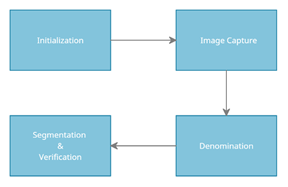
\includegraphics[width=8.5cm]{methodology.png}}
  \vspace{-3mm}
  %\centerline{(a) Result 1}\medskip
\end{minipage}
%
\caption{4-Part Process Pipeline}
\label{fig:methodology}
\vspace{-3mm}
\end{figure}

The method is divided into 4 parts as detailed in figure 1.

\subsection{Initialization}
The first step is to initialize benchmark values by processing sample images of multiple notes of each denomination. The values to test note denomination and security features are produced after processing each note of the same denomination. The respective values are averaged and multiple bell curves, similar to figure 2, are produced, where the mean serves as the benchmark value.

\begin{figure}[ht]

\begin{minipage}[b]{1.0\linewidth}
  \centering
  \centerline{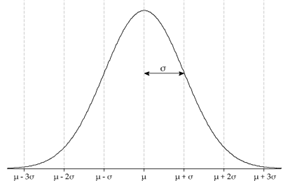
\includegraphics[width=8.5cm]{bell_curve.png}}
  \vspace{-3mm}
  %\centerline{(a) Result 1}\medskip
\end{minipage}
%
\caption{Bell-Curve}
\label{fig:bellcurve}
\vspace{-3mm}
\end{figure}

\newpage

\subsection{Image Capture}
The second step is to acquire a front-lit and back-lit image of the note that is passed into the automatic dispenser machine. The back-lit image is used to test the watermark, whereas the front-lit image is used to test the remaining security features. 

\subsection{Denomination}
Pakistani Notes have different sizes. Regions-of-interest can only be segmented and accurately tested after determining the denomination of a note. Hence, the third step is determining the bill denomination. There are a number of ways to determine the bill denomination; (a) Analyzing intensity histogram of note, (b) reading bill denomination from note, (c) reading denomination marker from note. We used method (a) because it was the simplest. The average intensity value of the note was found by analyzing the histogram of intensity values. The value was then compared with all the benchmark values for each denomination. If the average value was found to be within one standard deviation of the benchmark (mean) for any denomination, then that particular denomination was determined as the denomination of the received note. The above criteria were set such as to account for errors due to fading away of note color caused by age.

\subsection{Segmentation \& Verification}
\begin{figure}[h!]

\begin{minipage}[b]{1.0\linewidth}
  \centering
  \centerline{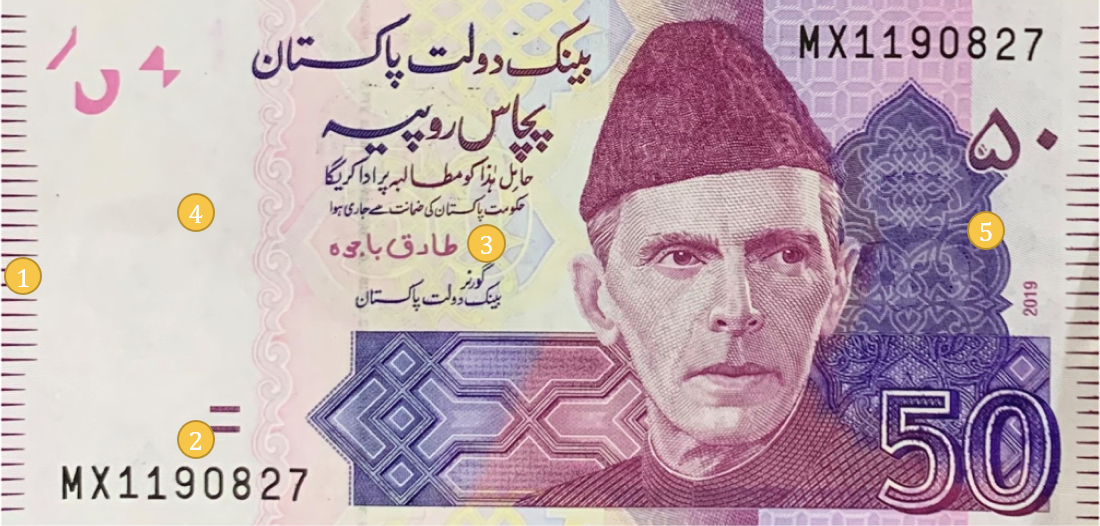
\includegraphics[width=8.5cm]{note.png}}
  \vspace{-3mm}
  %\centerline{(a) Result 1}\medskip
\end{minipage}
%
\caption{Features Segmented}
\label{fig:note}
\vspace{-3mm}
\end{figure}

The final step is to segment the regions-of- interests via predefined coordinates and verify the security feature listed in section 1 as seen in figure 3. After segmentation the regions-of-interest were converted to gray-scale. The process details are explained in section 3.

\subsubsection{Raised Lines on Note Edge}
The raised lines on the note edge are produced by the intaglio printing process. Intaglio printing is the opposite of relief printing, where the printing is done from ink that is below the surface of the plate. The design is cut, scratched, or etched into the printing surface or plate \cite{ScaleUp_MLSP:13}. It is not possible to test the raised printing without 3D imaging. However, we could count the number of raised lines present in the note. The line edges in the segmented region were detected via Sobel. Sobel worked the best because the lines were straight. Once line edges were detected, morphological processing was used to complete broken edges followed by filling. The connected components were then counted. If the line count was exactly 34 then the note would be accepted. The raised line count serves a good authentication indicator because all denominations of notes, except PKR 10, have the same number of raised lines. 

\subsubsection{Denomination Marker}
The notes denomination marker must match the determined denomination in section 2.3. For example, a PKR 50 note has 2 filled horizontal rectangles as the denomination marker. A PKR 100 note has 3. However, a PKR 1000 note has the same number of markers as PKR 50 note. The difference is that they are filled circles instead of rectangles. In addition to counting denomination markers via the process explained in section 2.4.1, their area was also extracted via region properties. If the total area of the denomination marker comes within 1 standard deviation of the mean of total area (figure 2 in section 2.1) for the determined denomination, then the note would be accepted. The Denomination marker count and its total area serves as an great authentication indicator, because all notes of the same denomination are identical, hence value for $\mathbf{\sigma}$ is very small.

\subsubsection{Governor’s Signature}
The signature verification was performed by checking for similarity between strokes. Canny edge detection was used to detect the signature edges. Canny worked best here because unlike Sobel, it can detect lines that a not straight to a good degree of accuracy. Disconnected edges were connected via morphological processing and filled. Next the boundaries function learned in the course lab was used to extract boundary pixels of each stroke. The signature function, also learned in lab, was then applied on the boundary of each stroke. The result of signature function is the distance of a boundary pixel from a centroid and the angle that the pixel and centroid make relative to an axis. The distance and angle values for every pixel were compared to their respective benchmark (mean). If all the values were within 1 standard deviation of their respective mean values (figure 2 in section 2.1), the then note was accepted. The signature serves as excellent authentication indicator, because all notes have identical signatures, hence the value for $\mathbf{\sigma}$ is very small.

\subsubsection{Watermark}
The watermark verification for a note of a particular denomination is performed simply by comparing the region with the respective pre-stored image. The watermark stands as the strongest visual indicators of a genuine note. It is produced at the time of printing by varying the thickness of the paper and can not be produced without the sophisticated printing machinery. The watermark can tried to be replicated via printing light edges but it can never be identical to an original one \cite{ScaleUp_MLSP:14}. The note was only accepted if the comparison results were within as small threshold. Since, all notes have identical watermarks the threshold value was really small.

\subsubsection{Latent Image of Note Denomination}
The latent image is very light, placed on top of a complex pattern, and can be only viewed from a particular orientation by the naked eye. Hence, it required a series morphological processes to extract the image. The edges of lines, of which the latent image is made of, are detected via Sobel. Sobel worked best because the lines were straight. Sobel edge detection not extracted the latent image whilst eliminating most of the complex background patterns/edges. After a few rounds of morphological processing the latent image was clearly visible. Region properties was then used to find the total area of the connected components in the latent image. If the total area was within the 1 standard deviation of the mean of total area (figure 2 in section 2.1) for the determined denomination, then the note was accepted. The latent image serves as an excelent authentication indicator because they are identical on notes of the same denomination, hence the value for $\sigma$ is really small.

\section{Experimentation \& Results}
\label{sec:resultsanddiscussion}
The methodology described in section 2 was implemented in MATLAB. Figure 4 demonstrates Image Capturing detailed in section 2.2.

\begin{figure}[h]
\begin{minipage}[b]{.48\linewidth}
  \centering
  \centerline{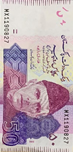
\includegraphics[width=2.0cm]{note1.png}}
  \centerline{(a)}%\medskip
  \vspace{-4mm}
\end{minipage}
\hfill
\begin{minipage}[b]{0.48\linewidth}
  \centering
  \centerline{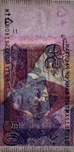
\includegraphics[width=2.0cm]{note2.png}}
  \centerline{(b)}%\medskip
  \vspace{-4mm}
\end{minipage}
\caption{Front-lit (a) and Back-lit (b) bills}
\label{fig:frontbacklit}
\vspace{-2mm}
\end{figure}
\newpage
However, due to lack of resources experimentation was limited to PKR 10, 50, 100 notes. The initial sample size for PKR 10 notes was 3, for PKR 50 was 4, and for PKR 100 was 2. Furthermore, the experimentation did not produce identical results for Denomination Markers, Governor's Signature, Watermark or the Latent Image for different notes of the same denomination. The reason being human error during Image Capture. The results, however were near identical and had larger standard deviations than expected but proved the validity of our methodology.

\subsection{Denomination Results}
\begin{figure}[ht]

\begin{minipage}[b]{1.0\linewidth}
  \centering
  \centerline{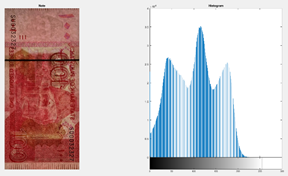
\includegraphics[width=8.5cm]{denomination1.png}}
  \vspace{-3mm}
  %\centerline{(a) Result 1}\medskip
\end{minipage}
%
\caption{Denomination Results on PKR 100 bill}
\label{fig:100rs}
\vspace{-3mm}
\end{figure}

\begin{figure}[ht]

\begin{minipage}[b]{1.0\linewidth}
  \centering
  \centerline{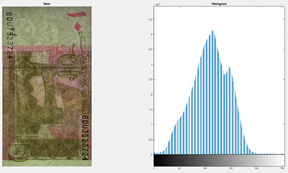
\includegraphics[width=8.5cm]{denomination2.png}}
  \vspace{-3mm}
  %\centerline{(a) Result 1}\medskip
\end{minipage}
%
\caption{Denomination Results on PKR 10 bill}
\label{fig:10rs}
\vspace{-3mm}
\end{figure}

\begin{figure}[h]
\begin{minipage}[b]{.48\linewidth}
  \centering
  \centerline{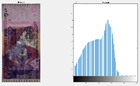
\includegraphics[width=4.0cm]{denomination3_1.png}}
  \centerline{}%\medskip
  \vspace{-4mm}
\end{minipage}
\hfill
\begin{minipage}[b]{0.48\linewidth}
  \centering
  \centerline{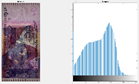
\includegraphics[width=4.0cm]{denomination3_2.png}}
  \centerline{}%\medskip
  \vspace{-4mm}
\end{minipage}
\caption{Denomination Results on PKR 50 bill}
\label{fig:50rs}
\vspace{-2mm}
\end{figure}
\newpage
Figures 5, 6 and 7 highlight the difference in intensity histograms for notes of different denomination. Figure 7 highlights the uniformity between intensity histograms of 2 different notes of the same denomination. The results prove that using the average intensity value to determine a notes denomination is a valid method.

\subsection{Raised Lines Results}

\begin{figure}[h!]

\begin{minipage}[b]{1.0\linewidth}
  \centering
  \centerline{
\includegraphics[width=8.5cm]{lines1.png}}
  \vspace{-3mm}
  %\centerline{(a) Result 1}\medskip
\end{minipage}
%
\caption{Grayscale Lines}
\label{fig:lines1}
\vspace{-3mm}
\end{figure}

\begin{figure}[h!]

\begin{minipage}[b]{1.0\linewidth}
  \centering
  \centerline{
\includegraphics[width=8.5cm]{lines2.png}}
  \vspace{-3mm}
  %\centerline{(a) Result 1}\medskip
\end{minipage}
%
\caption{Edge detected lines}
\label{fig:lines2}
\vspace{-3mm}
\end{figure}

\begin{figure}[h!]

\begin{minipage}[b]{1.0\linewidth}
  \centering
  \centerline{
\includegraphics[width=8.5cm]{lines3.png}}
  \vspace{-3mm}
  %\centerline{(a) Result 1}\medskip
\end{minipage}
%
\caption{Segmented Lines}
\label{fig:lines3}
\vspace{-3mm}
\end{figure}

Figure 8 shows the grayscale image of segmented region for Raised Lines present at the edge of a PKR 50 note. Figure 9 shows the region after applying Sobel edge detection. The region in figure 9 is closed via a square structuring element of size 4. The ‘bridge’ morphological operation is then applied. Then function imfill with parameter ‘holes’ is applied followed by dilation via the same structuring element as before. Finally, imfill with parameter ‘holes’ is applied again to produce the result in figure 10. Function bwlabel() is then used to count the connected components in figure 10 to produce a value for line count which is compared against the set criteria, as detailed in section 2.4.1. The results produced for other genuine notes were identical.

\subsection{Denomination Marker Results}
\begin{figure}[h!]

\begin{minipage}[b]{1.0\linewidth}
  \centering
  \centerline{
\includegraphics[width=3cm]{marker1.png}}
  \vspace{-3mm}
  %\centerline{(a) Result 1}\medskip
\end{minipage}
%
\caption{Edge detected denomination markers}
\label{fig:m1}
\vspace{-3mm}
\end{figure}

\begin{figure}[h!]

\begin{minipage}[b]{1.0\linewidth}
  \centering
  \centerline{
\includegraphics[width=3cm]{marker2.png}}
  \vspace{-3mm}
  %\centerline{(a) Result 1}\medskip
\end{minipage}
%
\caption{Segmented denomination markers}
\label{fig:m2}
\vspace{-3mm}
\end{figure}

Figure 11 is the result of applying Sobel edge detection to the segmented region of denomination markers of a PKR 50 note. Figure 10 was then closed via a structuring element of size 4. The ‘bridge’ morphological operation was applied followed by function imfill() with parameter ‘holes’ to produce the image in figure 12. Function bwlabel() was then used to count the number of denomination markers. For each connected component in figure 11 the area was found via the function regionprops() with parameter ‘Area’ The total area was compared against the criteria, as detailed in section 2.4.2. The results produced for notes of the same denomination were near identical.

\subsection{Governor’s Signature Results}
\begin{figure}[h!]

\begin{minipage}[b]{1.0\linewidth}
  \centering
  \centerline{
\includegraphics[width=5cm]{g1.png}}
  \vspace{-3mm}
  %\centerline{(a) Result 1}\medskip
\end{minipage}
%
\caption{Segmented signature}
\label{fig:g1}
\vspace{-3mm}
\end{figure}

\begin{figure}[h!]

\begin{minipage}[b]{1.0\linewidth}
  \centering
  \centerline{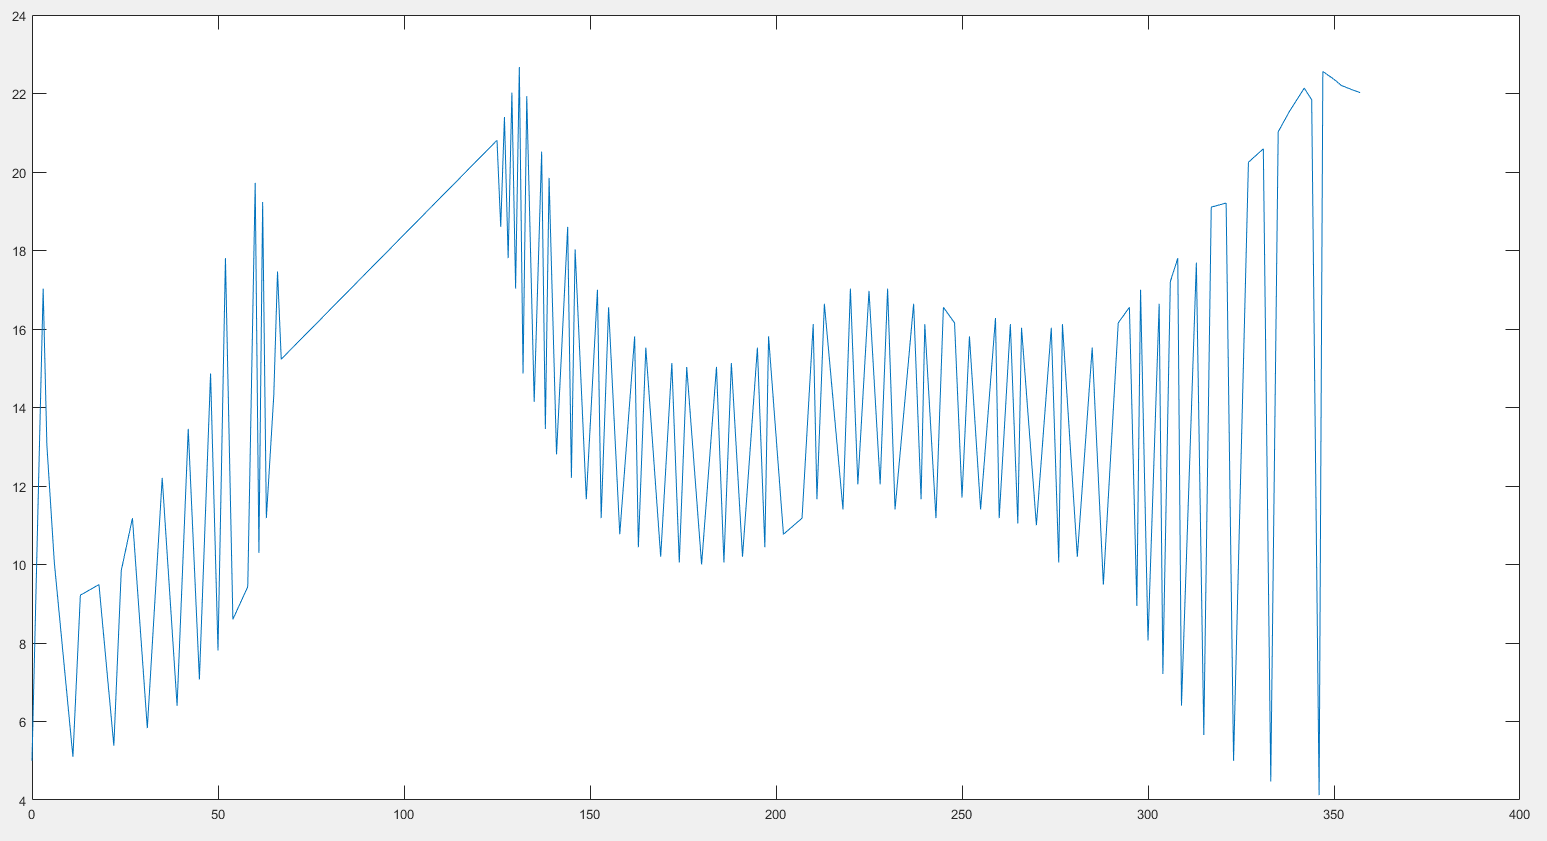
\includegraphics[width=8.5cm]{g2.png}}
  \vspace{-3mm}
  %\centerline{(a) Result 1}\medskip
\end{minipage}
%
\caption{Distance vs Angle plot for a stroke.}
\label{fig:g2}
\vspace{-3mm}
\end{figure}

\begin{figure}[h!]

\begin{minipage}[b]{1.0\linewidth}
  \centering
  \centerline{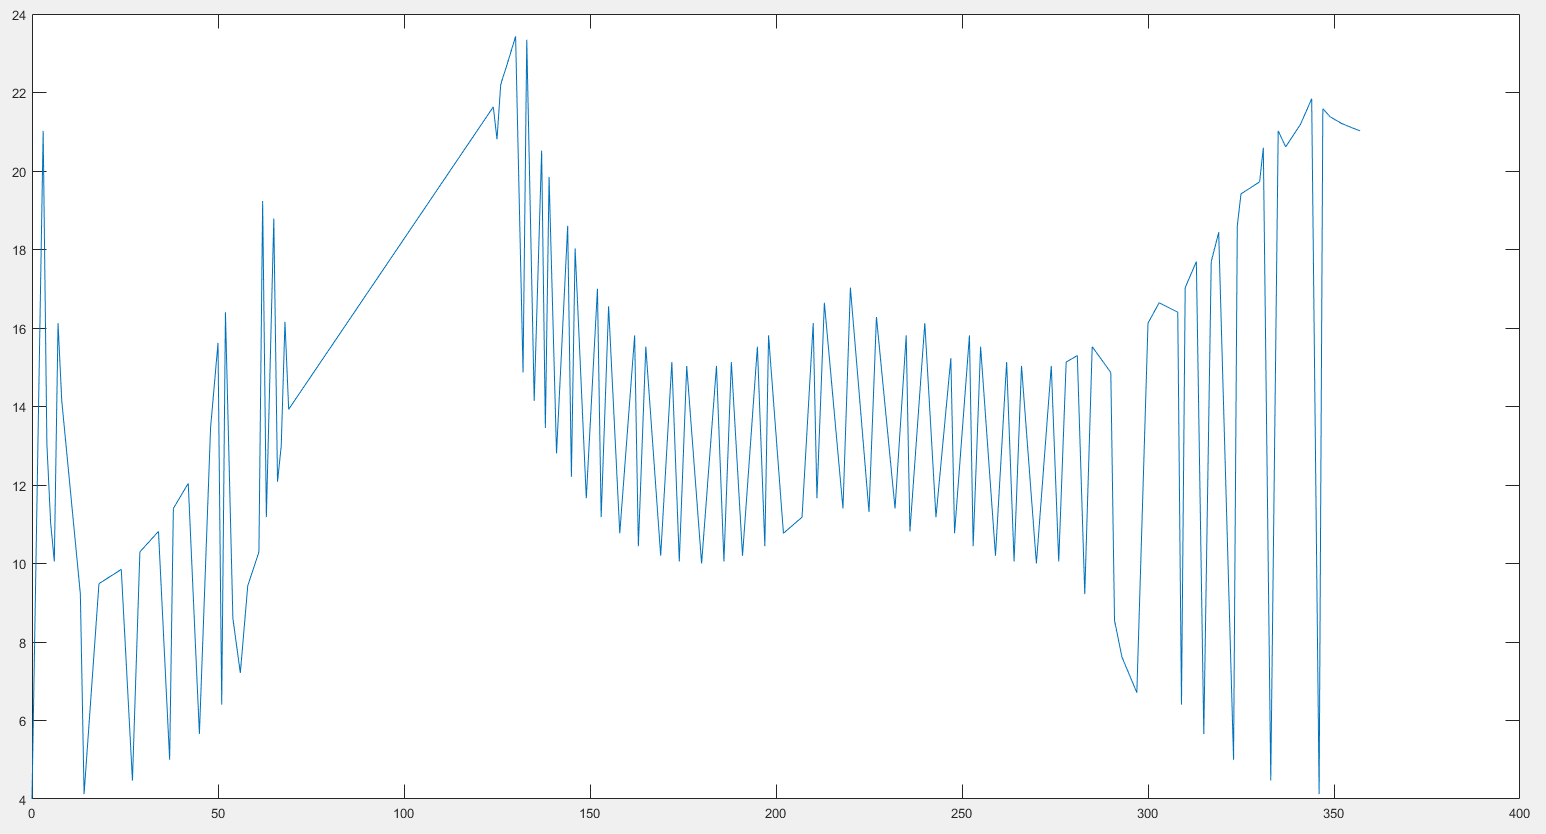
\includegraphics[width=8.5cm]{g3.png}}
  \vspace{-3mm}
  %\centerline{(a) Result 1}\medskip
\end{minipage}
%
\caption{Distance vs Angle plot for same stroke in another note.}
\label{fig:g3}
\vspace{-3mm}
\end{figure}
\newpage
The extracted signature region had its contrast adjusted via function imadjust(). The resulting image was thresholded at 0.33. Canny edge detection was applied to detect signature edges. The ‘bridge’ morphological operation was followed by imfill function with parameter ‘holes’. Finally, bwareaopen() was used with parameter 22 to produce the image in figure 12. The boundaries function with parameter 8 was applied to obtain boundary pixels for each stroke. The signature function was then used on each stroke to produce distance and angle values. Figure 14 and 15 highlight the uniformity between the strokes on 2 different and genuine PKR 50 notes. The results produced were expected to be identical given the uniformity of two different notes of the same denomination as explained in section 1. However, the slight discrepancy experienced in our experiment was due to human error as explained above. Nonetheless the results were near identical.
\newpage
\subsection{Watermark Results}
\begin{figure}[h!]

\begin{minipage}[b]{1.0\linewidth}
  \centering
  \centerline{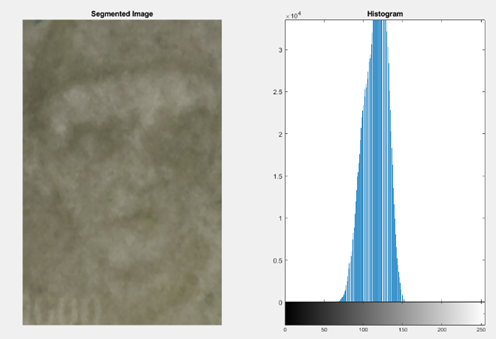
\includegraphics[width=8.5cm]{w1.png}}
  \vspace{-3mm}
  %\centerline{(a) Result 1}\medskip
\end{minipage}
%
\caption{Watermark region and histogram}
\label{fig:w1}
\vspace{-3mm}
\end{figure}

The extracted watermark region was subtracted from thee watermark regions in the stored samples as described in section 2.4.4. Function norm() was used to calculate the difference for each channel i.e red, green and blue. If the difference of each channel against the stored sample is within a certain threshold, then the bill passes the watermark comparison stage. The results for different notes of the same denomination were near identical.

\subsection{Latent Image of Note Denomination Results}

\begin{figure}[h!]

\begin{minipage}[b]{1.0\linewidth}
  \centering
  \centerline{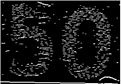
\includegraphics[width=5cm]{l1.png}}
  \vspace{-3mm}
  %\centerline{(a) Result 1}\medskip
\end{minipage}
%
\caption{Edges detected of latent image}
\label{fig:l1}
\vspace{-3mm}
\end{figure}

\begin{figure}[h!]

\begin{minipage}[b]{1.0\linewidth}
  \centering
  \centerline{
\includegraphics[width=5cm]{l2.png}}
  \vspace{-3mm}
  %\centerline{(a) Result 1}\medskip
\end{minipage}
%
\caption{Morphologically Processed Latent Image}
\label{fig:l2}
\vspace{-3mm}
\end{figure}

\begin{figure}[h!]

\begin{minipage}[b]{1.0\linewidth}
  \centering
  \centerline{
\includegraphics[width=5cm]{l3.png}}
  \vspace{-3mm}
  %\centerline{(a) Result 1}\medskip
\end{minipage}
%
\caption{Morphologically Processed Latent Image of the same note in a different orientation}
\label{fig:l3}
\vspace{-3mm}
\end{figure}
\newpage
Figure 17 was produced after applying Sobel edge detection after using imadjust() to correct contrast. The image was inverted and opened via a line structuring element of length 3. The opened image was reconstructed using the original inverted image. The image was then opened via a disk structuring element of size 8. Finally, the image was closed via another disk structuring element of size 10 to produce the result in figure 18. For each connected component function regionprops() with parameter ‘Area’ was used to find total area. The value was then compared with the criteria defined in section 2.4.5. The results for latent image were close but not near identical. The reason was human error as explained above. However, the discrepancy was amplified here due to multiple morphological processing steps that were used after trial and error. Figure 18 shows the result for the exact same PKR 50 note used to produce the result in figure 18. The difference was of small change in orientation. Hence, identical results can only be achieved here with the elimination of human error. 

\vspace{-1mm}
\section{Conclusion}
\label{sec:conclusion}
\vspace{-1mm}

A cheap alternative method for counterfeit currency detection in the scope of Pakistani Bank notes was presented in this paper. The methodology discussed in section 2 used the fact that all notes of the same denomination are identical and can be measured against a benchmark to test for genuineness. A statistical approach was employed to finding the benchmark for all tested features (figure 2 section 2.1). The experimental results in section 3 were satisfactory and proved the validity of the methodology discussed in section 2. The results can be further improved if the Image Capturing process is performed more accurately. Furthermore, the statistical accuracy of the algorithm can be improved greatly if every accepted bill is added to their respective sample list used to create benchmarks. Future work, can be based around improving the algorithm accuracy by focusing on the suggestions above.

%\vspace{-2mm}
%\section{Acknowledgments}
%\label{sec:majhead}
%%\vspace{-1mm}
%
%The authors thank Dr. Heikki Huttunen for valuable comments and Galilaeus Oy for kindly providing their experimental data. This work was financially supported by Finnish Programme for Centre of Excellence in Research 2006-2011, application no. 129657; the Academy of Finland, project no. 140018; and Tekes - the Finnish Funding Agency for Technology and Innovation, project DNo 700/31/2010. Support from Nokia Foundation is also acknowledged. 


%In LaTeX, to start a new column (but not a new page) and help balance the last-page column lengths, you can use the command ``$\backslash$pagebreak'' as demonstrated on this page (see the LaTeX source below).


% Below is an example of how to insert images. Delete the ``\vspace'' line,
% uncomment the preceding line ``\centerline...'' and replace ``imageX.ps''
% with a suitable PostScript file name.
% -------------------------------------------------------------------------

%\begin{figure}[htb]
%
%\begin{minipage}[b]{1.0\linewidth}
%  \centering
%  \centerline{\includegraphics[width=8.5cm]{image1}}
%%  \vspace{2.0cm}
%  \centerline{(a) Result 1}\medskip
%\end{minipage}
%%
%\begin{minipage}[b]{.48\linewidth}
%  \centering
%  \centerline{\includegraphics[width=4.0cm]{image3}}
%%  \vspace{1.5cm}
%  \centerline{(b) Results 3}\medskip
%\end{minipage}
%\hfill
%\begin{minipage}[b]{0.48\linewidth}
%  \centering
%  \centerline{\includegraphics[width=4.0cm]{image4}}
%%  \vspace{1.5cm}
%  \centerline{(c) Result 4}\medskip
%\end{minipage}
%%
%\caption{Example of placing a figure with experimental results.}
%\label{fig:res}
%%
%\end{figure}



% To start a new column (but not a new page) and help balance the last-page
% column length use \vfill\pagebreak.
% -------------------------------------------------------------------------
%\vfill
%\pagebreak




% References should be produced using the bibtex program from suitable
% BiBTeX files (here: strings, refs, manuals). The IEEEbib.bst bibliography
% style file from IEEE produces unsorted bibliography list.
% -------------------------------------------------------------------------
%\bibliographystyle{IEEEbib}
%\bibliography{IEEEabrv,ScaleUp_MLSP}

\renewcommand{\baselinestretch}{0.8}
\bibliographystyle{IEEEbib}
\small
\bibliography{IEEEabrv,ScaleUp_MLSP}
\renewcommand{\baselinestretch}{1}

\end{document}
